\chapter{Topology}

\begin{conv}
	Unless stated otherwise, assume these:
	\begin{convlist}
		\item $X$, $Y$ (and their sub-/super- scripts) will be topological spaces.
		
		\item Subsets of topological spaces will be considered under subspace topology.
		
		\item Product of topological spaces will be considered under the product topology.
		
		\item In a context, the ``parent'' totally ordered sets will be considered under as \LOTS's and their subsets under subspace topology (which is in general not the same as the topology from inherited order). (See \myRef{SEC: order topo}.)
		
		\item Monotonic functions will be assumed to be between \LOTS.
	\end{convlist}
\end{conv}



% needs more stuff
\section{Subspaces and Bases}

	\begin{lem}
		$\mathscr B$ is a base $\iff$ the arbitrary unions in $\mathscr B$ form a topology.\myMargin{``$\Rightarrow$'' requires \AC.}
	\end{lem}
	
	\begin{lem}\label{LEM: subspaces and bases}
		\leavevmode
		\begin{mylist}
			\item ``Being a subspace of'' is transitive.
			
			\item\label{LEMii: subspaces and bases} (Sub)base of a subspace can be obtained from that of the parent space.
		\end{mylist}
	\end{lem}
	
	
	
	
\section{Subsets of Topological Spaces}

	\begin{lem}\label{LEM: complements of clos and int}
		For any $A\subseteq X$, we have
		\begin{align*}
			X\setminus\clos A\phantom{^\circ} & = (X\setminus A)^\circ\text{, and}\\
			X\setminus A^\circ & = \phantom{(}\clos{X\setminus A}\text.
		\end{align*}
	\end{lem}
	
	\begin{proof}
		The first equality:
		\begin{subproof}
			``$\subseteq$'': Let $x\notin \clos A$. Thus we have an \onbd $U$ of $x$ that is disjoint from $A$, \ie, $U\subseteq X\setminus A\wimplies U\subseteq \RHS$.
		
			\noindent``$\supseteq$'': Let $x\in\RHS$ so that take an \onbd $U$ of $x$ contained in $X\setminus A$, \ie, $U$ doesn't intersect $A$ so that $x\notin \clos A$.\qedhere
		\end{subproof}
		
		The second follows if $A^\circ = X\setminus(\clos{X\setminus A})$. But by the first equality, $X\setminus(\clos{X\setminus A}) = (X\setminus(X\setminus A))^\circ\which = A^\circ$ as required.
	\end{proof}
	
	
	\begin{lem}\label{LEM: clos in subspaces}
		Let $A\subseteq X_1\subseteq X$. Then
		\begin{align*}
			\Cl_{X_1}(A) & = \Cl_X(A)\cap X_1\text{, and}\\
			\Int_{X_1}(A) & \supseteq \Int_X(A)\cap X_1\text.
		\end{align*}
	\end{lem}
	
	\begin{proof}
		$\Cl_X(A)\cap X_1$ is a closed set in $X_1$ containing $A$. Further, if $F$ is any closed set in $X$ such that $F\cap X_1\supseteq A$, then we need to show that $F\cap X_1\supseteq \RHS$. Indeed, since $F\supseteq A$, we have that $F\supseteq \Cl_X(A)\wimplies F\cap X_1\supseteq\Cl_X(A)\cap X_1$.
		
		Finally, since $\Int_X(A)\cap X_1$ is open in $X_1$ and is contained in $A$, the second inclusion follows.
	\end{proof}
	
	\begin{rmk}
		To show strict inclusion for $\Int$, consider $A = X_1 = \mathbb Q$ inside $X = \mathbb R$.
	\end{rmk}
	

	\begin{lem}\label{LEM: homeo img of clos and int}
		If $f\colon X\to Y$ is a \homeo, then for any $A\subseteq X$, we have
		\begin{align*}
			f(\clos A) & = \clos{f(A)}\text{, and}\\
			f(A^\circ) & = f(A)^\circ\text.
		\end{align*}
	\end{lem}
	
	\begin{proof}
		The first equality:
		\begin{subproof}
			``$\subseteq$'' is just restatement of \uline{$f$'s continuity}. Since \uline{$f^{-1}$ is also continuous}, we have $f^{-1}(\clos{f(A)})\subseteq \clos{f^{-1}(f(A))} = \clos A\wimplies \clos{f(A)}\subseteq f(\clos A)$, where we have also used \uline{bijectivity of $f$}.
		\end{subproof}
		
		The second equality is equivalent to showing that $Y\setminus f(A^\circ) = Y\setminus f(A)^\circ$. Indeed, $Y\setminus f(A^\circ) = f(X\setminus A^\circ) = f(\clos{X\setminus A}) = \clos{f(X\setminus A)} = \clos{Y\setminus f(A)} = Y\setminus f(A)^\circ$.
	\end{proof}
	



% add more stuff
\section{Functional Limits and Continuity}

	Let $E\subseteq X$ and $f\colon E\to Y$. Then for any $c\in X$ and $L\in Y$, we write \defn{$f(x)\to L$ as $x\to c$ in $X$} iff for every \onbd $V$ of $L$ in $Y$, there exists an \onbd $U$ of $c$ in $X$ such that $f(E\cap U\setminus\{c\})\subseteq V$. Note that ``in $X$'' is crucial and can't be dropped: Consider $f := \id$ on $(0, 1)$. Take $X_1$ to be the disjoint union topology of $(0, 1)$ and $\{1\}$ and $X_2 := (0, 1]$ under the subspace topology. Then $1$ is isolated in $X_1$ and thus $f(x)\to L$ for each $L\in (0, 1)$ as $x\to 1$ in $X_1$ (see \ref{LEMi: lims at isolated and lim pts} of \myRef{LEM: lims at isolated and lim pts}). \Otoh, $f(x)\to 1$ only as $x\to 1$ in $X_2$ since $1$ is a limit point of $(0, 1)$ in $X_2$ (see \ref{LEMii: lims at isolated and lim pts} of \myRef{LEM: lims at isolated and lim pts}).
	
	Intuitively, what this shows is that if $c$ is not already inside $E$, then the limits at $c$ depend on how $c$ and $E$ are embedded together in the ambient space:
	
	\begin{lem}[Tweaking ambient domains]\label{LEM: tweaking amb dom's}
		Assume the following:
		\begin{assmplist}
			\item $f\colon E\to Y$ where $E\subseteq F\which\subseteq X_1\cap X_2$.
			\item $F$ has the same subspace topology \wrt either $X_i$.
			\item $c\in F$ and $L\in Y$.
		\end{assmplist}
		Then $f(x)\to L$ as $x\to c$ in $X_1$ $\iff$ $f(x)\to L$ as $x\to c$ in $X_2$.
		\begin{center}
			\tikzset{every picture/.style={line width=0.75pt}} %set default line width to 0.75pt        
			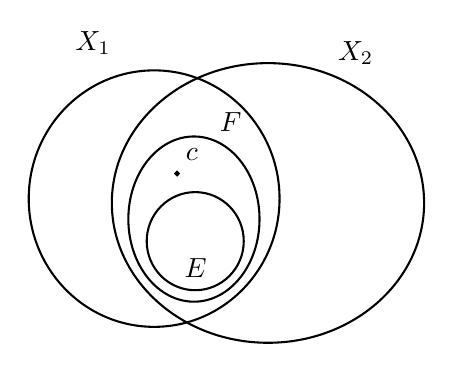
\begin{tikzpicture}[x=0.75pt,y=0.75pt,yscale=-1,xscale=1]
				%uncomment if require: \path (0,300); %set diagram left start at 0, and has height of 300
				%Shape: Ellipse [id:dp4107337296575948] 
				\draw   (81,129.54) .. controls (81,95.42) and (108.05,67.75) .. (141.42,67.75) .. controls (174.79,67.75) and (201.85,95.42) .. (201.85,129.54) .. controls (201.85,163.66) and (174.79,191.32) .. (141.42,191.32) .. controls (108.05,191.32) and (81,163.66) .. (81,129.54) -- cycle ;
				%Shape: Ellipse [id:dp7936945776152313] 
				\draw   (121.05,131.63) .. controls (121.05,94.43) and (154.73,64.26) .. (196.28,64.26) .. controls (237.82,64.26) and (271.5,94.43) .. (271.5,131.63) .. controls (271.5,168.84) and (237.82,199) .. (196.28,199) .. controls (154.73,199) and (121.05,168.84) .. (121.05,131.63) -- cycle ;
				%Shape: Ellipse [id:dp3956058502533526] 
				\draw   (137.85,150.04) .. controls (137.85,136.98) and (148.31,126.4) .. (161.22,126.4) .. controls (174.13,126.4) and (184.6,136.98) .. (184.6,150.04) .. controls (184.6,163.09) and (174.13,173.67) .. (161.22,173.67) .. controls (148.31,173.67) and (137.85,163.09) .. (137.85,150.04) -- cycle ;
				%Shape: Ellipse [id:dp8290181118038693] 
				\draw  [fill={rgb, 255:red, 0; green, 0; blue, 0 }  ,fill opacity=1 ] (151.67,117.45) .. controls (151.67,117) and (152.03,116.64) .. (152.48,116.64) .. controls (152.93,116.64) and (153.29,117) .. (153.29,117.45) .. controls (153.29,117.9) and (152.93,118.27) .. (152.48,118.27) .. controls (152.03,118.27) and (151.67,117.9) .. (151.67,117.45) -- cycle ;
				%Shape: Ellipse [id:dp18444722167504035] 
				\draw   (129,139.4) .. controls (129,117.42) and (143.15,99.6) .. (160.6,99.6) .. controls (178.05,99.6) and (192.2,117.42) .. (192.2,139.4) .. controls (192.2,161.38) and (178.05,179.2) .. (160.6,179.2) .. controls (143.15,179.2) and (129,161.38) .. (129,139.4) -- cycle ;
				
				% Text Node
				\draw (102.03,47.68) node [anchor=north west][inner sep=0.75pt]    {$X_{1}$};
				% Text Node
				\draw (228.53,52.47) node [anchor=north west][inner sep=0.75pt]    {$X_{2}$};
				% Text Node
				\draw (154.62,156.94) node [anchor=north west][inner sep=0.75pt]    {$E$};
				% Text Node
				\draw (155.26,104.08) node [anchor=north west][inner sep=0.75pt]    {$c$};
				% Text Node
				\draw (171.6,86.6) node [anchor=north west][inner sep=0.75pt]    {$F$};
			\end{tikzpicture}
		\end{center}
	\end{lem}
	
	\begin{proof}
		Just observe that if $U_1$ is an \onbd of $c$ in $X_1$, then $F\cap U_1$, being an \onbd of $c$ in $F$, is also equal to $F\cap U_2$ for some \onbd $U_2$ of $c$ in $X_2$. Also, since $E\subseteq F$, we also have $E\cap U_1 = E\cap U_2$.
	\end{proof}
	
	\begin{rmk}
		Thus, if $c\in E$ and the topology on $E$ is specified, then there's no need to talk of the ambient space at all, for there's a natural choice of the ambient space---$E$ itself!
	\end{rmk}
	
	\begin{lem}\label{LEM: lims at isolated and lim pts}
		\leavevmode
		\begin{mylist}
			\item\label{LEMi: lims at isolated and lim pts} All the codomain values are the limits of a function at an isolated point of the domain or of the ambient space.
			
			\item\label{LEMii: lims at isolated and lim pts} For Hausdorff codomains, there is at most one limit at a limit point of the domain.
		\end{mylist}
	\end{lem}
	
	\begin{proof}
		Let $f\colon E\to Y$ where $E\subseteq X$. Let $c\in X$.
		\begin{mylist}
			\item If $c$ is isolated in $E$ or in $X$, then there exists an \onbd $U$ of $c$ in $X$ such that $E\cap U \subseteq \{c\}$ so that for any open set $V$ in $Y$, we have $f(E\cap U\setminus\{c\}) = \emptyset\subseteq V$.
			
			\item Let $c$ be a limit point of $E$ and suppose $f(x)\to L_1, L_2$ as $x\to c$ for distinct $L_1$, $L_2$. Let $V_i$'s be opens separating $L_i$'s (since \uline{$Y$ Hausdorff}). Now, take \onbd{s} $U_i$'s of $c$ in $X$ such that $f(E\cap U_i\setminus\{c\})\subseteq V_i$. Now, $E\cap U_1\cap U_2\setminus\{c\}\ne\emptyset$ (since \uline{$c$ is a limit point of $E$}) which violates disjointness of $V_i$'s.\qedhere
		\end{mylist}
	\end{proof}
	
	\begin{rmk}
		Whenever the limit is unique \emph{and} the ambient space is clear (or instead, $c\in\dom f$ with the topology on $\dom f$ specified), we use the ``\defn{$\lim_{x\to c} f(x)$}'' notation.
	\end{rmk}
	
	
	\begin{lem}[Tweaking functional domains]\label{LEM: tweaking func doms}
		Assume the following:
		\begin{assmplist}
			\item $f\colon E\to Y$ and $g\colon F\to Y$ where $E\subseteq F\subseteq X$.
			\item $c\in X$ and $L\in Y$.
			\item $f$ and $g$ agree on $E$.
		\end{assmplist}
		Then \tfh:
		\begin{mylist}
			\item $g(x)\to L$ as $x\to c$ in $X$ $\implies$ $f(x)\to L$ as $x\to c$ in $X$.
			
			\item\label{LEMii: tweaking func doms} The converse holds if $E\supseteq U_0\cap F\setminus\{c\}$ for some \onbd $U_0$ of $c$.
		\end{mylist}
		\begin{center}
			\tikzset{every picture/.style={line width=0.75pt}} %set default line width to 0.75pt        
			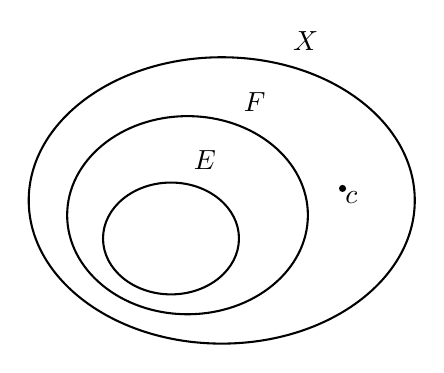
\begin{tikzpicture}[x=0.75pt,y=0.75pt,yscale=-1,xscale=1]
				%uncomment if require: \path (0,300); %set diagram left start at 0, and has height of 300
				%Shape: Ellipse [id:dp9131353224105325] 
				\draw   (110.5,125.01) .. controls (110.5,86.91) and (152.14,56.03) .. (203.5,56.03) .. controls (254.86,56.03) and (296.5,86.91) .. (296.5,125.01) .. controls (296.5,163.11) and (254.86,194) .. (203.5,194) .. controls (152.14,194) and (110.5,163.11) .. (110.5,125.01) -- cycle ;
				%Shape: Ellipse [id:dp5455521717188929] 
				\draw   (129.02,132.12) .. controls (129.02,105.77) and (154.98,84.4) .. (187.01,84.4) .. controls (219.04,84.4) and (245,105.77) .. (245,132.12) .. controls (245,158.48) and (219.04,179.85) .. (187.01,179.85) .. controls (154.98,179.85) and (129.02,158.48) .. (129.02,132.12) -- cycle ;
				%Shape: Ellipse [id:dp7957099753744543] 
				\draw   (146.3,143.34) .. controls (146.3,128.46) and (160.96,116.4) .. (179.05,116.4) .. controls (197.14,116.4) and (211.8,128.46) .. (211.8,143.34) .. controls (211.8,158.22) and (197.14,170.28) .. (179.05,170.28) .. controls (160.96,170.28) and (146.3,158.22) .. (146.3,143.34) -- cycle ;
				%Shape: Circle [id:dp42102133513485085] 
				\draw  [fill={rgb, 255:red, 0; green, 0; blue, 0 }  ,fill opacity=1 ] (260.53,119.23) .. controls (260.53,118.59) and (261.06,118.07) .. (261.7,118.07) .. controls (262.34,118.07) and (262.87,118.59) .. (262.87,119.23) .. controls (262.87,119.88) and (262.34,120.4) .. (261.7,120.4) .. controls (261.06,120.4) and (260.53,119.88) .. (260.53,119.23) -- cycle ;
				
				% Text Node
				\draw (236.35,42.28) node [anchor=north west][inner sep=0.75pt]    {$X$};
				% Text Node
				\draw (188.55,99.46) node [anchor=north west][inner sep=0.75pt]    {$E$};
				% Text Node
				\draw (212.62,71.61) node [anchor=north west][inner sep=0.75pt]    {$F$};
				% Text Node
				\draw (261.53,119.13) node [anchor=north west][inner sep=0.75pt]    {$c$};	
			\end{tikzpicture}
		\end{center}
	\end{lem}
	
	\begin{proof}
		Just note that for an \onbd $U$ of $c$, we have
		\begin{mylist}
			\item $f(U\cap E\setminus\{c\}) = g(U\cap E\setminus\{c\})\subseteq g(U\cap F\setminus\{c\})$; and
			
			\item $U\cap U_0$ is an \onbd of $c$ with $g(U\cap U_0\cap F\setminus\{c\}) \subseteq f(U\cap E\setminus \{c\})$.
			\qedhere
		\end{mylist}
	\end{proof}
	
	\begin{rmk}
		\begin{rmklist}
			\item The antecedent in the second claim formalizes that $E$ should be able to approximate $c$ at least as good as $F$; if $c\in F$, then it just says that $E$ contains a deleted \onbd of $c$ in $F$.
		
			\item To see the necessity of the antecendent, consider $x\mapsto 1/x$ with $E = \mathbb R^+$, $F = \mathbb R^*$, $X = \mathbb R$, and $Y = \extR$.
		\end{rmklist}
	\end{rmk}
	
	\begin{cor}
		\leavevmode
		\begin{mylist}
			\item Restricting the domain preserves continuity.
		
			\item Extending a continuous function by increasing its domain doesn't affect its continuity on the interior of the original smaller domain.
		\end{mylist}
	\end{cor}
	
	
	\begin{lem}[Tweaking codomains]
		Assume the following:
		\begin{assmplist}
			\item $f\colon E\to Y$ and $g\colon E\to Y_1$ where $E\subseteq X$ and $Y_1\supseteq Y$.
			\item $c\in X$ and $L\in Y$.
			\item $f$ and $g$ agree on $E$.
		\end{assmplist}
		Then $f(x)\to L$ as $x\to c$ in $X$ $\iff$ $g(x)\to L$ as $x\to c$ in $X$.
		\begin{center}
			\tikzset{every picture/.style={line width=0.75pt}} %set default line width to 0.75pt        
			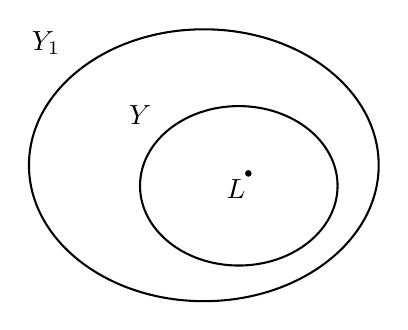
\begin{tikzpicture}[x=0.75pt,y=0.75pt,yscale=-1,xscale=1]
				%uncomment if require: \path (0,300); %set diagram left start at 0, and has height of 300
				
				%Shape: Ellipse [id:dp7493230657035939] 
				\draw  [color={rgb, 255:red, 0; green, 0; blue, 0 }  ,draw opacity=1 ] (100,136.5) .. controls (100,100.33) and (137.72,71) .. (184.25,71) .. controls (230.78,71) and (268.5,100.33) .. (268.5,136.5) .. controls (268.5,172.67) and (230.78,202) .. (184.25,202) .. controls (137.72,202) and (100,172.67) .. (100,136.5) -- cycle ;
				%Shape: Ellipse [id:dp73831363296357] 
				\draw  [color={rgb, 255:red, 0; green, 0; blue, 0 }  ,draw opacity=1 ] (153.5,146.41) .. controls (153.5,125.2) and (174.81,108) .. (201.09,108) .. controls (227.37,108) and (248.68,125.2) .. (248.68,146.41) .. controls (248.68,167.62) and (227.37,184.82) .. (201.09,184.82) .. controls (174.81,184.82) and (153.5,167.62) .. (153.5,146.41) -- cycle ;
				%Shape: Ellipse [id:dp35866211514698687] 
				\draw  [color={rgb, 255:red, 0; green, 0; blue, 0 }  ,draw opacity=1 ][fill={rgb, 255:red, 0; green, 0; blue, 0 }  ,fill opacity=1 ] (206.73,140.43) .. controls (206.73,139.83) and (206.27,139.35) .. (205.7,139.35) .. controls (205.13,139.35) and (204.67,139.83) .. (204.67,140.43) .. controls (204.67,141.02) and (205.13,141.5) .. (205.7,141.5) .. controls (206.27,141.5) and (206.73,141.02) .. (206.73,140.43) -- cycle ;
				
				% Text Node
				\draw (146.72,106.25) node [anchor=north west][inner sep=0.75pt]  [color={rgb, 255:red, 0; green, 0; blue, 0 }  ,opacity=1 ]  {$Y$};
				% Text Node
				\draw (99.88,70.72) node [anchor=north west][inner sep=0.75pt]    {$Y_{1}$};
				% Text Node
				\draw (193.72,141.77) node [anchor=north west][inner sep=0.75pt]    {$L$};
			\end{tikzpicture}
		\end{center}
	\end{lem}
	
	\begin{cor}
		Tweaking the codomain preserves continuity.
	\end{cor}
	
	
	\begin{prp}[Pointwise pasting]\label{PRP: pointwise pasting}
		Assume the following:
		\begin{assmplist}
			\item $f\colon E\to Y$ where $E\subseteq X$.
			\item $X$ is the union of finitely many $A_i\subseteq X$.
			\item $f|_i : E\cap A_i\to Y$.
			\item $c\in X$ and $L\in Y$.
			\item If $c\in A_i$, then $f|_i(x)\to L$ as $x\to c$ in $A_i$.
			\item Either $c\in\bigcap_i A_i$, or each $A_i$ is closed.
		\end{assmplist}
		Then $f(x)\to L$ as $x\to c$ in $X$.
		\begin{center}
			\tikzset{every picture/.style={line width=0.75pt}} %set default line width to 0.75pt        
			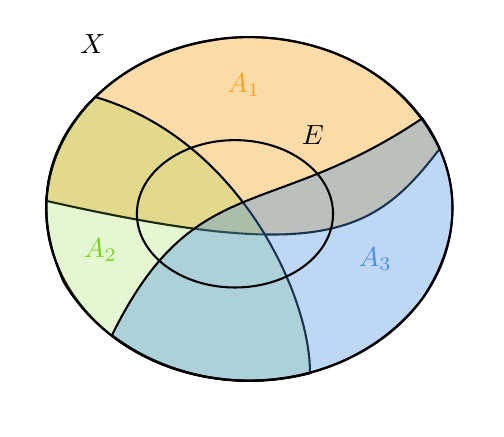
\begin{tikzpicture}[x=0.75pt,y=0.75pt,yscale=-1,xscale=1]
				%uncomment if require: \path (0,234); %set diagram left start at 0, and has height of 234
				%Shape: Arc [id:dp7257164231683342] 
				\draw  [draw opacity=0] (122.76,159.81) .. controls (118.6,150.61) and (116.32,140.62) .. (116.32,130.18) .. controls (116.32,84.45) and (160.12,47.37) .. (214.16,47.37) .. controls (254.14,47.37) and (288.52,67.67) .. (303.7,96.76) -- (214.16,130.18) -- cycle ; \draw  [color={rgb, 255:red, 0; green, 0; blue, 0 }  ,draw opacity=1 ] (122.76,159.81) .. controls (118.6,150.61) and (116.32,140.62) .. (116.32,130.18) .. controls (116.32,84.45) and (160.12,47.37) .. (214.16,47.37) .. controls (254.14,47.37) and (288.52,67.67) .. (303.7,96.76) ;  
				%Curve Lines [id:da5633899175715402] 
				\draw [fill={rgb, 255:red, 245; green, 166; blue, 35 }  ,fill opacity=0.4 ]   (116.46,126.29) .. controls (249.13,156.29) and (274.17,142.7) .. (305.85,101.21) .. controls (281.56,51.79) and (226.77,43.32) .. (196.76,48.85) .. controls (151.96,55.79) and (118.46,87.79) .. (116.46,126.29) -- cycle ;
				%Shape: Arc [id:dp4581318344087624] 
				\draw  [draw opacity=0] (243.92,209.09) .. controls (207.18,219) and (165.39,209.91) .. (139.11,183.34) .. controls (107.88,151.75) and (109.23,106.25) .. (140.08,76.07) -- (214.16,130.18) -- cycle ; \draw  [color={rgb, 255:red, 0; green, 0; blue, 0 }  ,draw opacity=1 ] (243.92,209.09) .. controls (207.18,219) and (165.39,209.91) .. (139.11,183.34) .. controls (107.88,151.75) and (109.23,106.25) .. (140.08,76.07) ;  
				%Shape: Arc [id:dp2032071512352036] 
				\draw  [draw opacity=0] (297.57,86.7) .. controls (322.61,121.13) and (314.68,166.8) .. (276.95,193.52) .. controls (238.88,220.49) and (183.72,218.78) .. (148.11,191.15) -- (214.16,130.03) -- cycle ; \draw  [color={rgb, 255:red, 0; green, 0; blue, 0 }  ,draw opacity=1 ] (297.57,86.7) .. controls (322.61,121.13) and (314.68,166.8) .. (276.95,193.52) .. controls (238.88,220.49) and (183.72,218.78) .. (148.11,191.15) ;  
				%Curve Lines [id:da2263394772216456] 
				\draw [color={rgb, 255:red, 0; green, 0; blue, 0 }  ,draw opacity=1 ][fill={rgb, 255:red, 126; green, 211; blue, 33 }  ,fill opacity=0.2 ]   (139.93,76.22) .. controls (209.31,96.51) and (243.6,171.9) .. (243.39,209.23) .. controls (197.76,220.8) and (148.19,204.71) .. (124.7,165.28) .. controls (113.15,139.09) and (109.79,105.66) .. (139.93,76.22) -- cycle ;
				%Curve Lines [id:da10665642138909104] 
				\draw [fill={rgb, 255:red, 74; green, 144; blue, 226 }  ,fill opacity=0.36 ]   (147.96,191.02) .. controls (187.32,111.33) and (223.48,136.26) .. (297.45,86.55) .. controls (321.13,120.48) and (312.19,151.4) .. (297.65,173.16) .. controls (263.73,217.96) and (194.4,226.16) .. (147.96,191.02) -- cycle ;
				%Shape: Ellipse [id:dp8801232310931526] 
				\draw   (160,132.5) .. controls (160,112.89) and (181.15,97) .. (207.25,97) .. controls (233.35,97) and (254.5,112.89) .. (254.5,132.5) .. controls (254.5,152.11) and (233.35,168) .. (207.25,168) .. controls (181.15,168) and (160,152.11) .. (160,132.5) -- cycle ;
				% Text Node
				\draw (202,63.4) node [anchor=north west][inner sep=0.75pt]  [color={rgb, 255:red, 245; green, 166; blue, 35 }  ,opacity=1 ]  {$A_{1}$};
				% Text Node
				\draw (133,142.73) node [anchor=north west][inner sep=0.75pt]  [color={rgb, 255:red, 126; green, 211; blue, 33 }  ,opacity=1 ]  {$A_{2}$};
				% Text Node
				\draw (265.33,147.4) node [anchor=north west][inner sep=0.75pt]  [color={rgb, 255:red, 74; green, 144; blue, 226 }  ,opacity=1 ]  {$A_{3}$};
				% Text Node
				\draw (131.17,44.73) node [anchor=north west][inner sep=0.75pt]    {$X$};
				% Text Node
				\draw (238,88.4) node [anchor=north west][inner sep=0.75pt]    {$E$};
			\end{tikzpicture}
		\end{center}
	\end{prp}
	
	\begin{proof}
		Let $V$ be an \onbd of $L$. Say $c\in A_i$'s and $c\notin A_j$'s. Thus, take \onbd{s} $U_i\cap A_i$ of $c$ in $A_i$ ($U_i$ open in $X_i$) such that $f|_i(U_i\cap E\cap A_i\setminus\{c\})\subseteq V$. Set $U := \bigl( \bigcap_i U_i \bigr)\cap \bigl(X\setminus \bigcup_j A_j\bigr)$\footnote{
			The second set in the union is motivated from the need to have $\bigcap_j X\setminus A_j$.
		} which is open since $i$'s and $j$'s are \uline{finitely many} and since onef \tfh{s}:
		\begin{mylist}
			\item \uline{$c$ is in each $A_k$} so that there are no $j$'s.
			\item \uline{Each $A_j$ is closed}.
		\end{mylist}
		Thus, $U$ is an \onbd of $c$ in $X$ with $f(U\cap E\setminus\{c\}) 
		= \bigl( \bigcup_i f(U\cap E\cap A_i\setminus\{c\}) \bigr)
			\cup \bigl( \bigcup_j f(U\cap E\cap A_j\setminus\{c\}) \bigr)
		\subseteq V\cup \emptyset = V$.
	\end{proof}
	
	\begin{rmk}
		\begin{mylist}
			\item Necessity of finitely many $A_i$'s: 
			Consider the function $f\colon \mathbb R^2\to\mathbb R$ given by $f(x, y) := x^2y/(x^4 + y^2)$ for $(x, y)\ne (0, 0)$ and $f(0, 0) := 0$. Along all the straight lines through origin (which are closed), $f(x)\to 0$ and yet $f$ has no limit at $(0, 0)$.\footnote{
				Consider evaluating along $y = mx^2$.
			} Note that here, $c\in \bigcap_i A_i$ \emph{and} each $A_i$ is closed.
			
			A much simpler example is to consider an infinite $X$ having at least one limit point and in which singletons are closed,\footnote{
				Such spaces are precisely the $T_1$ spaces. (See \myRef{LEM: t1 spaces}.)
			} and taking the codomain to be a Hausdorff space with at least two points.
			
			
			\item Necessity of ``$c\in\bigcap_i A_i$, or each $A_i$ closed'': Consider $f\colon \mathbb{R\to R}$ given by $f(x) := 0$ for $x < 0$ and $f(x) := 1$ for $x\ge 0$.
		\end{mylist}
	\end{rmk}
	
	\begin{cor}[Pasting lemma]
		If the domain is a finite union of closed sets on each of which the function's restriction is continuous, then the function is continuous.
	\end{cor}
	
	
	\begin{lem}\label{LEM: func lim => seq lims}
		Functional limits $\implies$ sequential limits.
	\end{lem}
	
	\begin{rmk}
		For taking sequential limits of a function at $c$, remember to have the sequence (eventually) not contain $c$!
	\end{rmk}
	
	\begin{proof}
		Let $f\colon E\to X$ where $E\subseteq X$ be such that $f(x)\to L$ as $x\to c$ for $c\in X$ and $L\in Y$. Let $x_i\to c$ for $(x_i)\in E\setminus\{c\}$. We show that $f(x_i)\to L$:
		\begin{subproof}
			Let $V$ be an \onbd of $L$. Take an \onbd $U$ of $c$ in $X$ such that $f(U\cap E\setminus\{c\})\subseteq V$. Now, $(x_i)$ eventually lies in $U$ and thus in $U\cap E\setminus\{c\}$ $\wimplies$ $(f(x_i))$ eventually lies in $V$.\qedhere
		\end{subproof}
	\end{proof}
	
	\begin{rmk}
		The converse holds for first-countable domains, but is false in general: See \myRef{PRP: continuity and closure in first countable} and the remark afterward.
	\end{rmk}
	
	\begin{cor}
		Continuity $\implies$ sequential continuity.
	\end{cor}
	
	
	\begin{lem}[Compositions and limits]
		Assume the following:
		\begin{assmplist}
			\item $f\colon E\to Y$ and $g\colon F\to Z$ where $E\subseteq X$ and $F\subseteq Y$.
			
			\item $f(E)\subseteq F$ and $f|\colon E\to f(E)$.
			
			\item $c\in X$, $L\in Y$ and $M\in Z$.
			
			\item $f(x)\to L$ as $x\to c$ in $X$.
			
			\item $g(y)\to M$ as $y\to L$ in $Y$.
			
			\item $L\in F\implies g(L) = M$.
		\end{assmplist}
		Then $(g\circ f|)(x)\to M$ as $x\to c$ in $X$.
		\begin{center}
			\tikzset{every picture/.style={line width=0.75pt}} %set default line width to 0.75pt        
			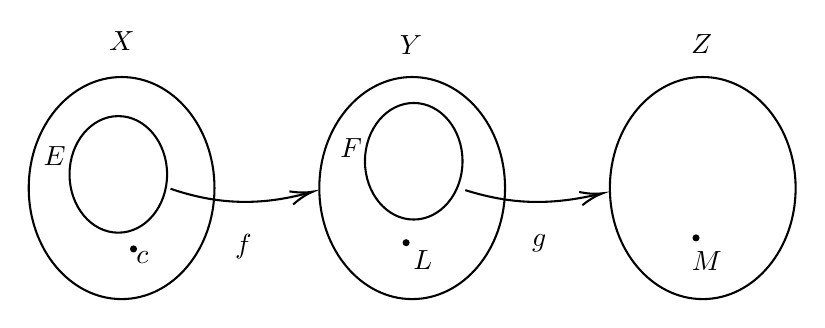
\begin{tikzpicture}[x=0.75pt,y=0.75pt,yscale=-1,xscale=1]
				%uncomment if require: \path (0,300); %set diagram left start at 0, and has height of 300
				%Shape: Ellipse [id:dp1747803797564662] 
				\draw   (70,143.5) .. controls (70,113.95) and (90.04,90) .. (114.75,90) .. controls (139.46,90) and (159.5,113.95) .. (159.5,143.5) .. controls (159.5,173.05) and (139.46,197) .. (114.75,197) .. controls (90.04,197) and (70,173.05) .. (70,143.5) -- cycle ;
				%Shape: Ellipse [id:dp6017870096769224] 
				\draw   (350,143.5) .. controls (350,113.95) and (370.04,90) .. (394.75,90) .. controls (419.46,90) and (439.5,113.95) .. (439.5,143.5) .. controls (439.5,173.05) and (419.46,197) .. (394.75,197) .. controls (370.04,197) and (350,173.05) .. (350,143.5) -- cycle ;
				%Shape: Ellipse [id:dp34515066020828034] 
				\draw   (210,143.5) .. controls (210,113.95) and (230.04,90) .. (254.75,90) .. controls (279.46,90) and (299.5,113.95) .. (299.5,143.5) .. controls (299.5,173.05) and (279.46,197) .. (254.75,197) .. controls (230.04,197) and (210,173.05) .. (210,143.5) -- cycle ;
				%Curve Lines [id:da6843663315256279] 
				\draw    (138.33,143.83) .. controls (160.43,151.41) and (181.14,152.36) .. (205.15,145.73) ;
				\draw [shift={(207,145.2)}, rotate = 163.81] [color={rgb, 255:red, 0; green, 0; blue, 0 }  ][line width=0.75]    (10.93,-3.29) .. controls (6.95,-1.4) and (3.31,-0.3) .. (0,0) .. controls (3.31,0.3) and (6.95,1.4) .. (10.93,3.29)   ;
				%Shape: Ellipse [id:dp7849282243502977] 
				\draw   (89.67,136.92) .. controls (89.67,121.41) and (100.19,108.83) .. (113.17,108.83) .. controls (126.15,108.83) and (136.67,121.41) .. (136.67,136.92) .. controls (136.67,152.43) and (126.15,165) .. (113.17,165) .. controls (100.19,165) and (89.67,152.43) .. (89.67,136.92) -- cycle ;
				%Shape: Ellipse [id:dp35883503443128895] 
				\draw   (232,130.58) .. controls (232,115.07) and (242.52,102.5) .. (255.5,102.5) .. controls (268.48,102.5) and (279,115.07) .. (279,130.58) .. controls (279,146.09) and (268.48,158.67) .. (255.5,158.67) .. controls (242.52,158.67) and (232,146.09) .. (232,130.58) -- cycle ;
				%Curve Lines [id:da7775078849380861] 
				\draw    (280.33,144.5) .. controls (302.43,151.42) and (320.98,151.98) .. (344.76,146.44) ;
				\draw [shift={(346.6,146)}, rotate = 166.33] [color={rgb, 255:red, 0; green, 0; blue, 0 }  ][line width=0.75]    (10.93,-3.29) .. controls (6.95,-1.4) and (3.31,-0.3) .. (0,0) .. controls (3.31,0.3) and (6.95,1.4) .. (10.93,3.29)   ;
				%Shape: Circle [id:dp8513976440995363] 
				\draw  [fill={rgb, 255:red, 0; green, 0; blue, 0 }  ,fill opacity=1 ] (119.33,172.83) .. controls (119.33,172.19) and (119.86,171.67) .. (120.5,171.67) .. controls (121.14,171.67) and (121.67,172.19) .. (121.67,172.83) .. controls (121.67,173.48) and (121.14,174) .. (120.5,174) .. controls (119.86,174) and (119.33,173.48) .. (119.33,172.83) -- cycle ;
				%Shape: Circle [id:dp7788897137688993] 
				\draw  [fill={rgb, 255:red, 0; green, 0; blue, 0 }  ,fill opacity=1 ] (250.67,169.83) .. controls (250.67,169.19) and (251.19,168.67) .. (251.83,168.67) .. controls (252.48,168.67) and (253,169.19) .. (253,169.83) .. controls (253,170.48) and (252.48,171) .. (251.83,171) .. controls (251.19,171) and (250.67,170.48) .. (250.67,169.83) -- cycle ;
				%Shape: Circle [id:dp4105766351501512] 
				\draw  [fill={rgb, 255:red, 0; green, 0; blue, 0 }  ,fill opacity=1 ] (390.33,167.5) .. controls (390.33,166.86) and (390.86,166.33) .. (391.5,166.33) .. controls (392.14,166.33) and (392.67,166.86) .. (392.67,167.5) .. controls (392.67,168.14) and (392.14,168.67) .. (391.5,168.67) .. controls (390.86,168.67) and (390.33,168.14) .. (390.33,167.5) -- cycle ;
				
				% Text Node
				\draw (107.33,66.73) node [anchor=north west][inner sep=0.75pt]    {$X$};
				% Text Node
				\draw (247.33,68.73) node [anchor=north west][inner sep=0.75pt]    {$Y$};
				% Text Node
				\draw (387.67,68.07) node [anchor=north west][inner sep=0.75pt]    {$Z$};
				% Text Node
				\draw (75.67,122.07) node [anchor=north west][inner sep=0.75pt]    {$E$};
				% Text Node
				\draw (218.67,118.07) node [anchor=north west][inner sep=0.75pt]    {$F$};
				% Text Node
				\draw (120.33,172.73) node [anchor=north west][inner sep=0.75pt]    {$c$};
				% Text Node
				\draw (253.83,172.07) node [anchor=north west][inner sep=0.75pt]    {$L$};
				% Text Node
				\draw (388,172.4) node [anchor=north west][inner sep=0.75pt]    {$M$};
				% Text Node
				\draw (168,164.4) node [anchor=north west][inner sep=0.75pt]    {$f$};
				% Text Node
				\draw (311,164.4) node [anchor=north west][inner sep=0.75pt]    {$g$};
			\end{tikzpicture}
		\end{center}
	\end{lem}
	
	\begin{proof}
		Let $W$ be an \onbd of $M$. Take an \onbd $V$ of $L$ such that $g(V\cap F\setminus\{L\})\subseteq W$ and an \onbd $U$ of $c$ such that $f(U\cap E\setminus\{c\})\subseteq V\cap F$ (since \uline{$f(E)\subseteq F$}). Because of \uline{the last assumption}, we have $(g\circ f)(U\cap E\setminus \{c\})\subseteq W$.
	\end{proof}
	
	\begin{rmk}
		To see the necessity of the last assumption, consider $f, g\colon[0, 1]\to[0, 1]$ given by $f := 1/2$ and $g := \delta_{1/2}$.
	\end{rmk}
	
	\begin{cor}
		Composition of continuous functions is continuous.
	\end{cor}





\section{Product Topology}

	From \ref{LEMii: subspaces and bases} of \myRef{LEM: subspaces and bases}, we immediately conclude:

	\begin{lem}
		Taking products and subspaces are compatible.
	\end{lem}
	
	\begin{rmk}
		This holds for box topology as well.
	\end{rmk}
	
	\begin{lem}\label{LEM: clos and prods commute}
		Closure of a product is the product of closures.
	\end{lem}
	
	\begin{proof}
		Let $A_i\subseteq X_i$. We show $\clos{\prod_i A_i} = \prod_i\clos{A_i}$.
		
		``$\subseteq$'': Suffice to show that $\prod_i F_i$ is closed for $F_i$'s closed in $X_i$'s. Let $(x_i)\notin\prod_i F_i$, say $x_{i_0}\notin F_{i_0}$. Then take an \onbd $U_{i_0}$ of $x_{i_0}$ disjoint from $F_{i_0}$. Now, $\pi_{i_0}^{-1}(U_{i_0})$ is an \onbd of $(x_i)$ that is disjoint from $\prod_i F_i$.
		
		``$\supseteq$'': Let $U := \bigcap_{j\in J}\pi_j^{-1}(U_j)$ be an \onbd of $(x_i)\in\RHS$, where $J$ is finite and each $U_j$ is open. Then each $U_j$ is an \onbd of $x_j$ and hence intersects $A_j$. Thus $U$ intersects $\prod_i A_i$.\myMargin{No choice \reqd.}
	\end{proof}
	
	\begin{rmk}
		The same holds for box topology as well; however \AC will be required for ``$\supseteq$''.
	\end{rmk}
	
	\begin{cor}
		Product of dense sets is dense in the product.
	\end{cor}
	
	\begin{rmk}
		This holds for box topology as well.
	\end{rmk}
	
	
	\begin{prp}[Convergence]\label{PRP: convergence in prod topo}
		Convergence in product topology is equivalent to convergence of each component sequence in the respective factor space.
	\end{prp}
	
	\begin{proof}
		``$\Rightarrow$'': Since projections are continuous.
		
		``$\Leftarrow$'': Let $X$ be the product of $X_i$'s and $x, (x^{(n)})\in X$ be such that $x^{(n)}_i\to x_i$ for each $i$. We show that $x^{(n)}\to x$. Let $U := \bigcap_j \pi_j^{-1}(U_j)$ be a basic \onbd of $x$ where $j$'s are finitely many. Thus, $(x^{(n)}_j)_n$ eventually lies in $U_j$ for each $j$. Since there are finitely many $j$'s, we conclude that $(x^{(n)})$ eventually lies in $U$.
	\end{proof}
	
	\begin{rmk}
		This does not hold for box topology: Consider the $\mathbb N$-fold product of discrete $\{0, 1\}$ endowed with box topology and consider the sequence whose $n$-th term is given by $(\underbrace{1, \ldots, 1}_\text{$n$ times}, 0, 0, \ldots)$.
	\end{rmk}	


\section{Order Topology}\label{SEC: order topo}
	
	If $X$ is totally ordered, then the \defn{order topology} on it is the one that's generated by open rays. The resulting space is called a \defn{linearly ordered topological space}, or \defn{\LOTS} in short.

	\begin{lem}[Immediate properties]\label{LEM: triv things on order topo}
		\leavevmode
		\begin{mylist}
			\item The base obtained from the subbase of open rays of a \LOTS $X$ comprises of the following sets:
			\begin{mylist}
				\item $(a, b)$;
				\item $[\min X, b)$ if $X$ has a minimum \elt;
				\item $(a, \max X]$ if $X$ has a maximum \elt; and,
				\item $[\min X, \max X]\which = X$ if $X$ has both, a maximum and a minimum.
			\end{mylist}
			
			\item Order topology is Hausdorff.
			
			\item A dense subset of a \LOTS is also topologically dense.
		\end{mylist}
	\end{lem}
	
	\begin{proof}
		\begin{mylist}
			\item It's easily shown that these sets form a base for $X$ and are generated by intersecting (at most two) open rays. Conversely, any open ray is generated by these basic sets:
			\begin{subproof}
				Let's show for right rays. In case there's a largest \elt, then $(a, +\infty) = (a, \max X]$. If not, then $(a, +\infty) = \bigcup_y (a, y)$.
			\end{subproof}
			
			\item Let $x < y$. If there's a $z$ between them, then $(-\infty, z)$ and $(z, +\infty)$ separate them. Otherwise, $(-\infty, y)$ and $(x, +\infty)$ do.
			
			\item Easily verified on basic opens.
			\qedhere
		\end{mylist}
	\end{proof}
	
	
	In an order topology, a point's isolated-ness is closely linked to the presence of its immediate successors and predecessors:
	
	%TODO: prettify
	\begin{lem}
		The isolated points in an order topology are precisely the following:
		\begin{mylist}
			\item An \elt that is least as well as greatest.
			\item A least \elt with an immediate successor.
			\item A greatest \elt with an immediate predecessor.
			\item An \elt with an immediate succesor and an immediate predecessor.
		\end{mylist}
		
		Thus, an order topology is discrete $\iff$ each non-least \elt has an immediate predecessor and each non-greatest \elt has an immediate successor.
	\end{lem}
	
	
	\begin{lem}[Subspaces and order]\label{LEM: subspaces of ord spaces}
		Topology induced from inherited order is coarser than the subspace topology. The two are distinct if and only if there exists an $x\in X\setminus Y$ such that one of \tfh{s}:
		\begin{mylist}
			\item There exists a $y\in Y\cap(x, +\infty)$ such that $Y\cap(-\infty, y)$ is nonemtpy, has no maximum \elt, and is strictly bounded above by $x$.
			\begin{center}
				\tikzset{every picture/.style={line width=0.75pt}} %set default line width to 0.75pt        
				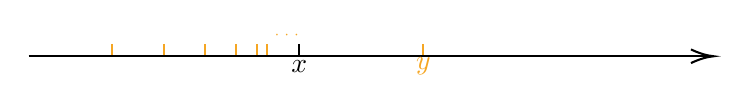
\begin{tikzpicture}[x=0.75pt,y=0.75pt,yscale=-1,xscale=1]
					%uncomment if require: \path (0,83); %set diagram left start at 0, and has height of 83
					%Straight Lines [id:da01936853933129612] 
					\draw    (240,36) -- (240,42) ;
					%Straight Lines [id:da8844525977816171] 
					\draw [color={rgb, 255:red, 245; green, 166; blue, 35 }  ,draw opacity=1 ]   (300,36) -- (300,42) ;
					%Straight Lines [id:da548768591837862] 
					\draw [color={rgb, 255:red, 245; green, 166; blue, 35 }  ,draw opacity=1 ][line width=0.75]    (220,36) -- (220,42) ;
					%Straight Lines [id:da15789047762154906] 
					\draw [color={rgb, 255:red, 245; green, 166; blue, 35 }  ,draw opacity=1 ][line width=0.75]    (210,36) -- (210,42) ;
					%Straight Lines [id:da8490513162935942] 
					\draw [color={rgb, 255:red, 245; green, 166; blue, 35 }  ,draw opacity=1 ][line width=0.75]    (195,36) -- (195,42) ;
					%Straight Lines [id:da04447043781483084] 
					\draw [color={rgb, 255:red, 245; green, 166; blue, 35 }  ,draw opacity=1 ][line width=0.75]    (175,36) -- (175,42) ;
					%Straight Lines [id:da9546042987546921] 
					\draw [color={rgb, 255:red, 245; green, 166; blue, 35 }  ,draw opacity=1 ][line width=0.75]    (150,36) -- (150,42) ;
					%Straight Lines [id:da9775801599544265] 
					\draw [color={rgb, 255:red, 245; green, 166; blue, 35 }  ,draw opacity=1 ][line width=0.75]    (225,36) -- (225,42) ;
					%Straight Lines [id:da27116758097643756] 
					\draw    (110,42) -- (438,42) ;
					\draw [shift={(440,42)}, rotate = 180] [color={rgb, 255:red, 0; green, 0; blue, 0 }  ][line width=0.75]    (10.93,-3.29) .. controls (6.95,-1.4) and (3.31,-0.3) .. (0,0) .. controls (3.31,0.3) and (6.95,1.4) .. (10.93,3.29)   ;
					
					% Text Node
					\draw (226.67,28.73) node [anchor=north west][inner sep=0.75pt]  [font=\tiny,color={rgb, 255:red, 245; green, 166; blue, 35 }  ,opacity=1 ]  {$\cdots $};
					% Text Node
					\draw (235,42.4) node [anchor=north west][inner sep=0.75pt]    {$x$};
					% Text Node
					\draw (295.17,41.07) node [anchor=north west][inner sep=0.75pt]  [color={rgb, 255:red, 245; green, 166; blue, 35 }  ,opacity=1 ]  {$y$};
				\end{tikzpicture}
			\end{center}
			
			\item There exists a $y\in Y\cap (-\infty, x)$ such that $Y\cap (y, +\infty)$ is noempty, has no minumum \elt, and is strictly bounded below by $x$.
			\begin{center}
				\tikzset{every picture/.style={line width=0.75pt}} %set default line width to 0.75pt        
				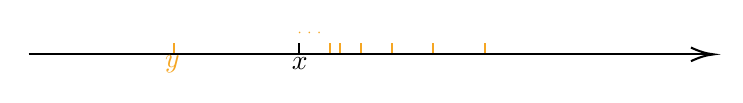
\begin{tikzpicture}[x=0.75pt,y=0.75pt,yscale=-1,xscale=1]
					%uncomment if require: \path (0,81); %set diagram left start at 0, and has height of 81
					%Straight Lines [id:da18221030232000857] 
					\draw    (237,44.33) -- (237,38.33) ;
					%Straight Lines [id:da3691657875978427] 
					\draw [color={rgb, 255:red, 245; green, 166; blue, 35 }  ,draw opacity=1 ]   (177,44.33) -- (177,38.33) ;
					%Straight Lines [id:da7358981130075375] 
					\draw [color={rgb, 255:red, 245; green, 166; blue, 35 }  ,draw opacity=1 ][line width=0.75]    (257,44.33) -- (257,38.33) ;
					%Straight Lines [id:da1570573797633832] 
					\draw [color={rgb, 255:red, 245; green, 166; blue, 35 }  ,draw opacity=1 ][line width=0.75]    (267,44.33) -- (267,38.33) ;
					%Straight Lines [id:da1337557688432529] 
					\draw [color={rgb, 255:red, 245; green, 166; blue, 35 }  ,draw opacity=1 ][line width=0.75]    (282,44.33) -- (282,38.33) ;
					%Straight Lines [id:da33855001471610024] 
					\draw [color={rgb, 255:red, 245; green, 166; blue, 35 }  ,draw opacity=1 ][line width=0.75]    (302,44.33) -- (302,38.33) ;
					%Straight Lines [id:da711745352779275] 
					\draw [color={rgb, 255:red, 245; green, 166; blue, 35 }  ,draw opacity=1 ][line width=0.75]    (327,44.33) -- (327,38.33) ;
					%Straight Lines [id:da2349411084918449] 
					\draw [color={rgb, 255:red, 245; green, 166; blue, 35 }  ,draw opacity=1 ][line width=0.75]    (252,44.33) -- (252,38.33) ;
					%Straight Lines [id:da5203095744994863] 
					\draw    (107,44) -- (435,44) ;
					\draw [shift={(437,44)}, rotate = 180] [color={rgb, 255:red, 0; green, 0; blue, 0 }  ][line width=0.75]    (10.93,-3.29) .. controls (6.95,-1.4) and (3.31,-0.3) .. (0,0) .. controls (3.31,0.3) and (6.95,1.4) .. (10.93,3.29)   ;
					
					% Text Node
					\draw (250,36.93) node [anchor=north west][inner sep=0.75pt]  [font=\tiny,color={rgb, 255:red, 245; green, 166; blue, 35 }  ,opacity=1 ,rotate=-180]  {$\cdots $};
					% Text Node
					\draw (171.17,43.07) node [anchor=north west][inner sep=0.75pt]  [color={rgb, 255:red, 245; green, 166; blue, 35 }  ,opacity=1 ]  {$y$};
					% Text Node
					\draw (232.33,44.07) node [anchor=north west][inner sep=0.75pt]    {$x$};
				\end{tikzpicture}
			\end{center}
		\end{mylist}
		
		Thus, the topologies match if $Y$ is convex or dense in $X$.
	\end{lem}
	
	\begin{proof}
		It's straightforward to verify that the enumerated conditions are equivalent to saying that $Y\cap (x, +\infty)$, and \resp $Y\cap (-\infty, x)$, are not open in the order topology. Since the open rays indeed generate the order topology, this shows the ``if and only iff'' part.
		
		Finally, note that if $Y$ is convex or dense in $X$, then none of the conditions can arise, and we are done.
	\end{proof}
	
	\begin{rmk}
		Consider $\{-1\}\cup(0, 1]\subseteq \mathbb R$, where the two topologies are distinct.
	\end{rmk}
	
	
	Using \myRef{LEM: tweaking amb dom's} and \myRef{LEM: tweaking func doms}, one immediately gets:
	
	\begin{lem}[One-sided limits]
		Assume the following:
		\begin{assmplist}
			\item $X$ is a \LOTS.
			\item $f\colon E\to Y$ where $E\subseteq X$.
			\item $c\in X$ and $L\in Y$.
			\item $g\colon E\cap(-\infty, c]\to Y$ and $h\colon E\cap(-\infty, c)\to Y$ are restrictions of $f$.
		\end{assmplist}
		Then \tfae:
		\begin{mylist}
			\item $g(x)\to L$ as $x\to c$ in $X$.
			\item $g(x)\to L$ as $x\to c$ in $(-\infty, c]$.
			\item $h(x)\to L$ as $x\to c$ in $X$.
			\item $h(x)\to L$ as $x\to c$ in $(-\infty, c]$.
		\end{mylist}
		
		Similarly, we have the ``right-sided'' version.
	\end{lem}
	
	We use ``\defn{$f(x)\to L$ as $x\to c^\pm$ in $X$}'' to denote the above equivalent statements. Note that here, instead of ``in $X$'', we could've chosen ``in $(-\infty, c]$'' or \resp, ``in $[c, +\infty)$''. \myRef{PRP: pointwise pasting} readily yields:
	
	\begin{lem}\label{LEM: limits via the left and right hand limits}
		Assume the following:
		\begin{assmplist}
			\item $X$ is a \LOTS.
			\item $f\colon E\to Y$ where $E\subseteq X$.
			\item $c\in X$ and $L\in Y$.
		\end{assmplist}
		Then \tfae:
		\begin{mylist}
			\item $f(x)\to L$ as $x\to c$ in $X$.
			
			\item $f(x)\to L$ as $x\to c^+$ and as $x\to c^-$ in $X$.
		\end{mylist}
	\end{lem}
	
	
	\begin{prp}\label{PRP: one-sided lims of monotonics}
		Assume the following:
		\begin{assmplist}
			\item $X$, $Y$ are \LOTS's.
			\item $f\colon E\to Y$ where $E\subseteq X$.
			\item $f$ is increasing.
			\item $c\in X$.
		\end{assmplist}
		Then, \tfh:
		\begin{alignat*}{2}
			f(x)& \to_\If \sup f(E\cap (-\infty, c)) &&\text{ as $x\to c^-$ in $X$}\\
			f(x)& \to_\If \inf f(E\cap (c, +\infty)) &&\text{ as $x\to c^+$ in $X$}
		\end{alignat*}
		We similarly have a dual version for decreasing $f$.
	\end{prp}
	
	\begin{proof}
		Let $f$ be increasing. The proof for decreasing $f$ would be similar. We show only the first statement, second's proof being similar. Let $f(E\cap (-\infty, c))$ have the \lub, say $\alpha$. We need to show that $f|(x)\to \alpha$ as $x\to c$ in $X$, where $f|\colon E\cap (-\infty, c)\to Y$. Let $J$ be a basic \onbd of $\alpha$. We have two cases:
		\begin{mylist}
			\item $\alpha$ is the least \elt of $Y$: Then $f(E\cap (-\infty, c)\cap (-\infty, \infty)) = f(E\cap (-\infty, c))\subseteq \{\alpha\}\subseteq J$.
			
			\item $\alpha$ is not the least \elt: Then \wlogg, let $J$'s left end be open, say at $y \which < \alpha$. Thus, take an $x\in E\cap (-\infty, c)$ such that $f(x) > y$. Now, since $f$ is \uline{increasing}, $f(E\cap (-\infty, c)\cap (x, +\infty))\which = f(E\cap (x, c))\subseteq (y, \alpha]\subseteq J$.
			\qedhere
		\end{mylist}
	\end{proof}
	
	\begin{cor}\label{COR: one-sided lims of monotonics in a complete codom}
		Monotonics taking values in a complete codomain admit one-sided limits at all points of the domain.
	\end{cor}
	
	\begin{proof}
		Let $f\colon X\to Y$ be increasing and $c\in X$. We find a left-side limit $L$ at $c$. We have two cases:
		\begin{mylist}
			\item $c$ is not the least \elt of $X$: Then $f((-\infty, c))$ is nonempty and bounded above by $f(c)$, so we may take $L$ to be its \lub\ (which exists since \uline{$Y$ is complete}).
			
			\item $c$ is the least \elt of $X$: Then the domain of $f|\colon(-\infty, c)\to Y$ is empty and thus we may take $L$ to be any point in $Y$.
		\end{mylist}
		The proofs for other cases are similar.
	\end{proof}
	
	\begin{rmk}
		To see the necessity of well-definedness of \RHS in \myRef{PRP: one-sided lims of monotonics} and that of completeness in \myRef{COR: one-sided lims of monotonics in a complete codom}, consider $f\colon \mathbb R\to\mathbb R\setminus\{0\}$ given by
		\[
		f(x) := 
		\begin{cases}
			x, & x < 0\\
			x + 1, & x \ge 0
		\end{cases}\text.
		\]
	\end{rmk}
	
	
	\begin{prp}[Continuity and monotonicity]
		\leavevmode
		\begin{mylist}
			\item Strictly monotonic surjections are homeomorphisms.
			
			\item A monotonic surjection is continuous provided the codomain's order is dense.
		\end{mylist}
	\end{prp}
	
	\begin{proof}
		\begin{mylist}
			\item Since inverses of strictly monotonic bijections are strict monotones as well, it suffices to show openness, which is easy to verify.
			
			\item Let $X$, $Y$ be \LOTS's and $f\colon X\to Y$ be an increasing surjection. The proof for decreasing $f$ would be similar. Let $J$ be a basic open set of $Y$. We show that $f^{-1}(J)$ is open. Start with an $x\in f^{-1}(J)$, \ie, $f(x)\in J$. The following cases arise:
			\begin{mylist}
				\item $f(x)$ is the least in $Y$: Then $J = [f(x), y)$ for some $y > f(x)$. Due to \uline{denseness} and \uline{surjectivity}, take $b\in X$ such that $f(x) < f(b) < y$. Since $f$ is \uline{increasing}, we have $x < b$ and $f([x, b))\subseteq [f(x), f(b)] \subseteq [f(x), y) = J$. Since $f((-\infty, x]) = \{f(x)\}$ (as \uline{$f(x)$ is the least element}), we have that $f((-\infty, b))\subseteq J$ so that $(-\infty, b)$ works.
				
				\item $f(x)$ is the greatest in $Y$: \Lly as above.
				
				\item $f(x)$ is neither: Then \wlogg, take $J = (y_1, y_2)$ for $y_1 < f(x) < y_2$. Due to \uline{denseness} and \uline{surjectivity}, take $a, b\in X$ such that $y_1 < f(a) < f(x) < f(b) < y_2$. Again, since $f$ is \uline{increasing}, $a < x < b$ and $f((a, b))\subseteq [f(a), f(b)]\subseteq (y_1, y_2) = J$ so that $(a, b)$ works.
				\qedhere
			\end{mylist}
		\end{mylist}
	\end{proof}
	
	\begin{rmk}
		\begin{mylist}
			\item Necessity of surjectivity: $f\colon \mathbb{R\to R}$ given by $f(x) := x$ for $x < 0$ and $f(x) := x + 1$ for $x\ge 0$.
			
			\item Necessity of denseness of codomain: Consider the sign function $\mathbb R\to \{-1, 0, 1\}$.
		\end{mylist}
	\end{rmk}
	
	
	\begin{prp}[Monotone convergence]\label{PRP: monotone convg}
		Let $X$ be a \LOTS and $(x_i)\in X$ be increasing (\resp decreasing). Let $L\in X$. Then $x_i\to L$ $\iff$ $L = \sup_i x_i$ (\resp $L = \inf_i x_i$).
	\end{prp}
	
	\begin{proof}
		We show for increasing $(x_i)$.
		
		``$\Rightarrow$'': We show that $L$ is the supremum of $x_i$'s:
		\begin{prooflist}
			\item It's an \ub: If not, then we can take an $x_N > L$ so that $(x_i)$ eventually lies out of $(-\infty, x_N)$, an \onbd of $L$.
			
			\item It's the \lub: If $M < L$, then $(x_i)$ eventually lies in the \onbd $(M, +\infty)$ of $L$, so that $M$ can't be an \ub for $(x_i)$.
		\end{prooflist}
		
		``$\Leftarrow$'': Let $I$ be a basic \onbd of $L$. We have two cases:
		\begin{mylist}
			\item $L$ is the least \elt: Then each $x_i = L$.
			\item $L$ is not the least \elt: Then \wlogg, let $I$'s left end be open, say at $a\which < L$. Thus, take $x_N > a$, so that for each $i\ge N$, we have $x_i\in (a, L]\which\subseteq I$.\qedhere
		\end{mylist}
	\end{proof}
	
	
	
	\begin{lem}[$\liminf$ and $\limsup$]
		Let $X$ be a \LOTS and $(x_i)\in X$. Then there exists at most one $L^+\in X$ such that for any $a\in X$, \tfh:
		\begin{mylist}
			\item $a > L^+$ $\implies$ $x_i$'s are evetually all less than $a$.
			\item $a < L^+$ $\implies$ infinitely many $x_i$'s are greater than $a$.
		\end{mylist}
		A dual statement holds for ``$L^-$''.
	\end{lem}
	
	\begin{proof}
		We only show for ``$L^+$''. Suppose $L^+_1$ and $L^+_2$ are such with $L^+_1 < L^+_2$. We have two cases:
		\begin{mylist}
			\item $a\in (L^+_1, L^+_2)$: Then $x_i$'s are eventually all less than $a$ (since $a > L^+_1$), contradicting that infinitely many $x_i$'s are greater than $a$ (since $a < L^+_2$).
			
			\item $(L^+_1, L^+_2) = \emptyset$: Then $x_i$'s are eventually all less than $L^+_2$ (since $L^+_2 > L^+_1$), and hence, less than or equal to $L^+_1$, contradicting that infinitely many $x_i$'s are greater than $L^+_1$ (since $L^+_1 < L^+_2$).
			\qedhere
		\end{mylist}
	\end{proof}
	
	\begin{rmk}
		This allows to use the ``\defn{$\limsup_i x_i$}'' and ``\defn{$\liminf_i x_i$}'' notations.
	\end{rmk}
	
	
	\begin{lem}[Chracterizing $\limsup$ and $\liminf$]
		Let $X$ be a complete \LOTS and $(x_i)\in X$ be bounded. Then
		\begin{align*}
			\textstyle \limsup_i x_i & = \textstyle\inf_i \sup_{j\ge i} x_j\text{, and}\\
			\textstyle\liminf_i x_i & = \textstyle\sup_i \inf_{j\ge i} x_j \text{.}
		\end{align*}
	\end{lem}
	
	\begin{proof}
		Define $x_i^+ := \sup_{j\ge i} x_j$ and $x_j^- := \inf_{j\ge i} x_j$, which are well-defined since $X$ is complete and $(x_i)$ bounded. We only show that $\limsup_i x_i = \inf_i x_i^+$:
		\begin{prooflist}
			\item Let $a > \inf_i x_i^+$. Then some $x_N^+ < a$ so that $x_i\le x_N^+ < a$ for each $i\ge N$.
			
			\item Let $a < \inf_i x_i^+$ and $N$ be any index. Then $a < x_N^+$ so that there exists an $i\ge N$ such that $x_i > a$.\qedhere
		\end{prooflist}
	\end{proof}
	
	
	\begin{lem}
		Let $X$ be a \LOTS and $(x_i), (y_i)\in X$. Then \tfh:
		\begin{mylist}
			\item $\liminf_i x_i\le_\If\limsup_i x_i$.
			\item Each $x_i\le y_i$ $\implies$ $\liminf_i x_i\le_\If\liminf_i y_i$ and $\limsup_i x_i\le_\If\limsup_i y_i$.
		\end{mylist}
	\end{lem}
	
	\begin{proof}
		We'll use the notations $L^\pm_x$ and $L^\pm_y$.
		\begin{mylist}
			\item Suppose $L^+_x < L^-_x$. Two cases are there:
			\begin{mylist}
				\item $a\in (L^+_x, L^-_x)$: Then $x_i$'s are eventually all less than $a$ (since $a > L^+_x$) and greater than $a$ (since $a < L^-_x$), a contradiction.
				
				\item $(L^+_x, L^-_x) = \emptyset$: Then $x_i$'s are evetually all less than $L^-_x$ (since $L^-_x > L^+_x$) and hence, less than or equal to $L^+_x$, contradicting that $x_i$'s are eventually all greater than $L^+_x$ (since $L^+_x < L^-_x$).
			\end{mylist}
			
			
			\item We'll only show $L^-_x\le L^-_y$. Suppose not. Again two cases:
			\begin{mylist}
				\item $a\in (L^-_y, L^-_x)$: Then $x_i$'s are eventually all greater than $a$ (since $a < L^-_x$) and there are infinitely many $y_i$'s less than $a$ (since $a > L^-_y$). But this then means that $y_i < a < x_i$ for some $i$.
				
				\item $(L^-_y, L^-_x) = \emptyset$: Then $x_i$'s are eventually all greater than $L^-_y$ (since $L^-_y < L^-_x$) and hence, greater than or equal to $L^-_x$. Also, there are infinitely many $y_i$'s less than $L^-_x$ (since $L^-_x > L^-_y$). But this means that $y_i < L^-_x\le x_i$ for some $i$.
				\qedhere
			\end{mylist}
		\end{mylist}
	\end{proof}
	
	
	\begin{prp}
		Let $X$ be a LOTS and $(x_i), L\in X$. Then $\lim_i x_i = L\iff \limsup_i x_i = L = \liminf_i x_i$.
	\end{prp}
	
	\begin{proof}
		``$\Rightarrow$'': If $a > L$, then $(x_i)\in (-\infty, a)$ evetually. If $a < L$, then $(x_i)\in (a, +\infty)$ eventually.
		
		``$\Leftarrow$'': Let $I$ be an \onbd of $L$. The following cases arise:
		\begin{mylist}
			\item $L$ is not the greatest of the least \elt: Then, \wlogg, take $I = (a, b)$. Now, $x_i$'s are eventually all less than $b$ (since $b > L \which = \limsup_i x_i$) and also greater than $a$ (since $a < L\which = \liminf_i x_i$). Thus, eventually, $(x_i)\in (a, b) = I$.
			
			\item The rest of the cases, when $L$ is greatest or least, are done \lly.\qedhere
		\end{mylist}
	\end{proof}
	
	
	Note that $\limsup, \liminf, \lim\colon X^\mathbb N\rightharpoonup X$ are not continuous unless $|X| = 1$, for in every nonempty basic open, there exists a sequence that converges to any given \elt of $X$. However, we have:
	
	\begin{prp}
		For a \LOTS $X$ and $n\ge 1$, the functions $\max, \min\colon X^n\to X$ are continuous.
	\end{prp}
	
	\begin{proof}
		We show for $\max$. Let $x\in X^n$ and $I$ be an \onbd of $\max(x)$. We have the following cases:
		\begin{mylist}
			\item $\max(x)$ is the least in $X$: Then each $x_i = \max(x)$ so that $\max(I\times\cdots\times I)\subseteq I$.
			
			\item $\max(x)$ is not the least: Then \wlogg, let $I$'s left end be open, say at $a$. Set $b := \max\bigl(\{a, x_1, \ldots, x_n\}\setminus\{\max(x)\}\bigr)$. We have two cases:
			\begin{mylist}
				\item $c\in (b, \max(x))$: Then define
				\begin{align*}
					J_i & :=
					\begin{cases}
						(c, +\infty)\cap I, & x_i = \max(x)\\
						(c, -\infty), & x_i < \max(x)
					\end{cases}
					\intertext{
				\item $(b, \max(x)) = \emptyset$: Then define
						}
					J_i & :=
					\begin{cases}
						(b, +\infty)\cap I, & x_i = \max(x)\\
						(-\infty, \max(x)), & x_i < \max(x)
					\end{cases}\\
					& \which = 
					\begin{cases}
						[\max(x), +\infty)\cap I, & x_i = \max(x)\\
						(-\infty, b], & x_i < \max(x)
					\end{cases}
				\end{align*}
			\end{mylist}
			In either case, we have $\max(\prod_i J_i)\subseteq I$.\qedhere
		\end{mylist}
	\end{proof}
	



\section{Denseness}

	\begin{lem}\label{LEM: denseness is transitive}
		``Being dense'' is transitive.
	\end{lem}
	
	\begin{proof}
		Let $A\subseteq B\subseteq X$ with $A$ dense in $B$ and $B$ dense in $X$. Let $U$ be a nonempty open in $X$. Then \uline{$B$ being dense}, intersects $U$ so that $U\cap B$ is a nonempty open in $B$ and thus is intersected by the \uline{dense $A$} $\wimplies$ $A$ intersects $U$.
	\end{proof}
	
	
	\begin{lem}\label{LEM: cont img of dense is dense}
		Continuous image of dense is dense in the image.
	\end{lem}
	
	\begin{proof}
		Let $f\colon X\to Y$ be surjective continuous and $A\subseteq X$ be dense in $X$. Then $\clos{f(A)}\supseteq f(\clos A) = f(X) = Y$.
	\end{proof}
	
	
	
	\begin{lem}\label{LEM: dense on a subset}
		Let $A, B\subseteq X$. Then \tfh:
		\begin{mylist}
			\item $B\cap A$ is dense in $B$ $\implies$ $B\subseteq \clos A$.
			
			\item\label{LEMii: dense on a subset} The converse holds if $B$ is open.
		\end{mylist}
	\end{lem}
	
	\begin{proof}
		\begin{mylist}
			\item We have $B = \Cl_B(B\cap A)\subseteq B\cap \clos{B\cap A}\subseteq\clos{B\cap A}\subseteq\clos A$.
			
			\item We need to show that $\Cl_B(B\cap A) = B$. Indeed, if $F$ is any closed such that $B\cap A\subseteq B\cap F$, then $B\subseteq F$ (otherwise, take $x\in B\setminus F\wimplies x\in B\setminus A\wimplies x\in B\setminus \clos A$ for \uline{$B$ is open}, contradicting $B\subseteq \clos A$).\qedhere
		\end{mylist}
	\end{proof}
	
	\begin{rmk}
		To see the necessity of openness of $B$ in \ref{LEMii: dense on a subset}, consider $A = \{1, 1/2, \ldots\}$ and $B = \{0\}$.
	\end{rmk}
	
	
	
\subsection{Nowhere dense sets}
	
	\myRef{LEM: dense on a subset} gives insight as to why nowhere dense sets are called so---they are dense on no nonempty \emph{open} set. On the other hand, dense sets are dense on the whole space.
	
	\begin{lem}
		Let $U$ be open in $X$ and $A\subseteq X$. Then \tfae:
		\begin{mylist}
			\item $U\subseteq \clos A$.
			
			\item Every nonempty open subset contained in $U$ intersects $\clos A$.
			
			\item Every nonempty open subset contained in $U$ intersects $A$.
		\end{mylist}
	\end{lem}
	
	\begin{cor}\label{COR: characterizing nowhere dense}
		\Tfae for a subset $A$ of $X$:
		\begin{mylist}
			\item $X\setminus \overline A$ is dense.
			
			\item $A$ is nowhere dense.
			
			\item Each nonempty open set contains a nonemtpy open subset disjoint from $\overline A$.
			
			\item Each nonempty open set contains a nonemtpy open subset disjoint from $A$.
		\end{mylist}
	\end{cor}
	
	Subsets of a topological space that are countable unions of nowhere dense sets are called \defn{first category} or \defn{meagre} sets. Others are called \defn{second category} sets.
	
	\begin{rmk}
		In $\mathbb R$:\footnote{Nonmeagre-ness can be concluded by Baire's category theorem (\myRef{THM: BCT}).}
		\begin{center}
			\begin{tabular}{r|cc}
				& meagre & nonmeagre\\
				\hline
				dense & $\mathbb Q$ & $\mathbb R$\\
				nondense & $\emptyset$ & $[0, 1]$
			\end{tabular}
		\end{center}
	\end{rmk}
	
	\begin{lem}
		If $F_1, F_2, \ldots$ are closed in $X$ with $X\setminus\bigcup_i F_i$ dense, then each $F_i$ is nowhere dense.
	\end{lem}
	
	\begin{rmk}
		Baire's category theorem (\myRef{THM: BCT}) gives a converse to above, stating that complements of meagre sets are dense in a complete metric space.
	\end{rmk}
	
	\begin{prp}\label{PRP: versions of BCT}
		In a topological space, \tfae:
		\begin{mylist}
			\item\label{PRPi: versions of BCT} Complements of meagre sets are dense.
			\item\label{PRPii: versions of BCT} Countable intersections of open dense sets are dense.
		\end{mylist}
	\end{prp}
	
	\begin{proof}
		`` $\Rightarrow$ '': Let $U_1, U_2, \cdots$ be open dense. Now, $\bigcap_i U_i \which= X\setminus\bigcup_i(X\setminus U_i)$ is dense if each $X\setminus U_i$ is nowhere dense $\wimpliedby$ $X\setminus(\overline{X\setminus U_i})\which= U_i$ (since \uline{$U_i$ open}) is \uline{dense}, which is true.
		
		`` $\Leftarrow$ '': Let $A_1, A_2, \ldots$ be nowhere dense. Then each $X\setminus\overline A_i$ is dense $\wimplies$ $\bigcap_i(X\setminus \overline A_i)\which= X\setminus\bigcup_i\overline A_i$ is dense $\wimplies$ $X\setminus\bigcup_i A_i$ is dense as well, being a larger set.
	\end{proof}
	
	
	
	
\section{Connectedness}\label{SEC: connectedness}

	A subset $E$ of $X$ is said to be \defn{disconnected} iff there exist disjoint open sets $U$, $V$ together containing $E$, and each a having nonempty intersection with $E$. If $E$ is not disconnected, we call it \defn{connected}. $X$ is called \defn{totally disconnected} iff the only connected subsets of it are singletons.
	
	\begin{lem}
		Discrete spaces are totally disconnected.
	\end{lem}

	\begin{lem}[Characterizing disconnectedness]
		$E\subseteq X$ is disconnected $\iff$ $E$ can be written as a union of two nonempty subsets $A$, $B$ of $X$ such that $\overline A\cap B = \emptyset = A\cap\overline B$.
	\end{lem}
	
	\begin{proof}
		``$\Rightarrow$'': Take $U$, $V$ open in $X$ such that $E\cap U$, $E\cap V$ are nonempty, $E\subseteq U\cup V$, and $E\cap U\cap V = \emptyset$. Now put $A := E\cap U$ and $B := E\cap V$. Then $\overline A\cap B\subseteq \overline{E\cap U}\cap V = \emptyset$.
		
		``$\Leftarrow$'': Take $U := X\setminus \overline A$ and $V := X\setminus \overline B$. Then $B\subseteq U$ and $A\subseteq V$ so that both are nonempty and $E\subseteq U\cup V$. Also, $E\cap U\cap V = E\setminus(\overline A\cup\overline B) = \emptyset$.
	\end{proof}
	
	% tags:
	%		- order topology
	%		- connectedness
	\begin{prp}[Linear continua are connected]\label{PRP: linear continua are connected}
		The connected subsets of a dense and complete \LOTS\myMargin{
			Can we improve to partial orders?
		} are precisely its convex subsets.\footnote{
			Recall that a convex subset of an ordered set is any set $I$ such that $[x, y]\subseteq I$ whenever $x, y\in I$ with $x\le y$.
		}
	\end{prp}
	
	\begin{proof}
		Let $X$'s topology come from a dense and complete total order. Suppose $I\subseteq X$ is convex, and yet separated by opens $U$, $V$. Take $a\in U\cap I$ and $b\in V\cap I$. \Wlogg, assume $a < b$ (\uline{the order is total}) so that $[a, b]\subseteq I$ (since \uline{$I$ is convex}). Note that $U$, $V$ also form a separation of $[a, b]$. Since $U\cap [a, b]$ is nonempty and bounded, let $c$ be its \uline{l.u.b.} Clearly, $c\in[a, b]$ so that there are two cases:
		\begin{mylist}
			\item[$c\in U$:]
			Take a basic open interval $J\subseteq U$ containing $c$. 
			Note that $c < b$ (otherwise, $c = b\which\in V$) so that we may assume that $J$ is open at its right end, say $d$.
			Note that $d \le b$ (otherwise, $b\in (c, d)\which\subseteq J\which\subseteq U$).
			Now, $c < d$ and yet, there can't be any \elt between $c$ and $d$:
			\begin{subproof}
				Such an \elt would be in $U\cap[a, b]$ (being in $J$ and in $(c, b)$) despite being strictly greater than $c$.
			\end{subproof}
			\begin{center}
				\tikzset{every picture/.style={line width=0.75pt}} %set default line width to 0.75pt        
				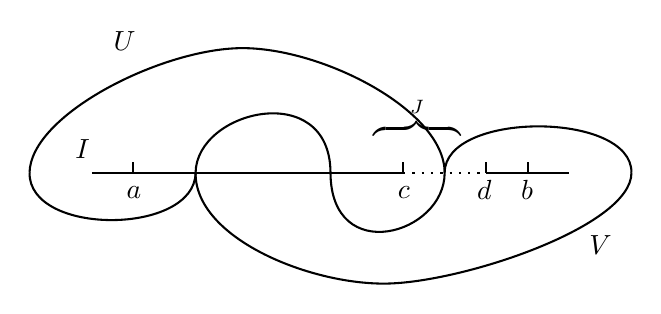
\begin{tikzpicture}[x=0.75pt,y=0.75pt,yscale=-1,xscale=1]
					%uncomment if require: \path (0,286); %set diagram left start at 0, and has height of 286
					%Straight Lines [id:da13873956932151277] 
					\draw    (100,110) -- (250,110) ;
					%Curve Lines [id:da5026608886419746] 
					\draw    (70,110) .. controls (69.6,140.6) and (149.6,140.2) .. (150,110) .. controls (150.4,79.8) and (214.8,64.6) .. (215,110) .. controls (215.2,155.4) and (270,139.8) .. (270,110) .. controls (270,80.2) and (360.4,80.2) .. (360,110) ;
					%Curve Lines [id:da2896370855379784] 
					\draw    (70,110) .. controls (70.4,82.6) and (131.2,51.4) .. (170,50) .. controls (208.8,48.6) and (270,79.4) .. (270,110) ;
					%Curve Lines [id:da9844335844869916] 
					\draw    (150,110) .. controls (149.6,141.4) and (204.8,163.8) .. (241.6,163.4) .. controls (278.4,163) and (360,135.8) .. (360,110) ;
					%Straight Lines [id:da7723028029840726] 
					\draw    (120,105) -- (120,110) ;
					%Straight Lines [id:da735907602505697] 
					\draw    (310,105) -- (310,110) ;
					%Straight Lines [id:da702942107145262] 
					\draw    (250,105) -- (250,110) ;
					%Straight Lines [id:da8464971154904155] 
					\draw  [dash pattern={on 0.84pt off 2.51pt}]  (250,110) -- (290,110) ;
					%Straight Lines [id:da7444776708741307] 
					\draw    (290,105) -- (290,110) ;
					%Straight Lines [id:da6163612959884488] 
					\draw    (290,110) -- (330,110) ;
					
					% Text Node
					\draw (90.6,92.6) node [anchor=north west][inner sep=0.75pt]    {$I$};
					% Text Node
					\draw (115.27,115) node [anchor=north west][inner sep=0.75pt]    {$a$};
					% Text Node
					\draw (305.4,112) node [anchor=north west][inner sep=0.75pt]    {$b$};
					% Text Node
					\draw (246,115) node [anchor=north west][inner sep=0.75pt]    {$c$};
					% Text Node
					\draw (284.13,112) node [anchor=north west][inner sep=0.75pt]    {$d$};
					% Text Node
					\draw (234,72.07) node [anchor=north west][inner sep=0.75pt]    {$\overbrace{\quad \quad \quad \thinspace }^{J}$};
					% Text Node
					\draw (109,40.6) node [anchor=north west][inner sep=0.75pt]    {$U$};
					% Text Node
					\draw (338.2,138.8) node [anchor=north west][inner sep=0.75pt]    {$V$};
				\end{tikzpicture}
			\end{center}
			
			\item[$c\in V$:]
			Take a basic open interval $J\subseteq V$ containing $c$. 
			This time, $c > a$ (otherwise, $c = a\which\in U$) so that we may assume that $J$ is open at its left end, say $d$. But then, $d$ is an \ub for $U\cap[a, b]$ despite being strictly smaller than $c$:
			\begin{subproof}
				If $x > d$, then either $x\in (d, c]\which\subseteq J\which\subseteq V$; or $x > c\wimplies x\notin U\cap[a, b]$.
			\end{subproof}
			\begin{center}
				\tikzset{every picture/.style={line width=0.75pt}} %set default line width to 0.75pt        
				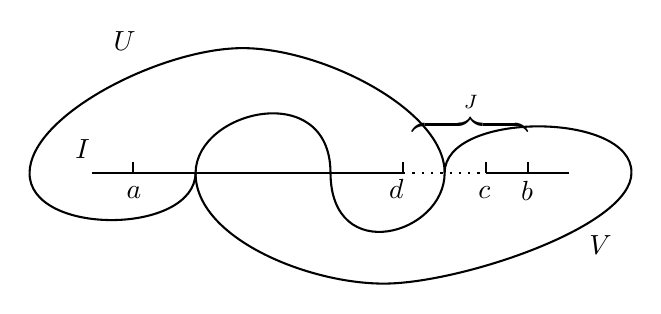
\begin{tikzpicture}[x=0.75pt,y=0.75pt,yscale=-1,xscale=1]
					%uncomment if require: \path (0,300); %set diagram left start at 0, and has height of 300
					
					%Straight Lines [id:da5516767296673053] 
					\draw    (120,130) -- (270,130) ;
					%Curve Lines [id:da884496609730284] 
					\draw    (90,130) .. controls (89.6,160.6) and (169.6,160.2) .. (170,130) .. controls (170.4,99.8) and (234.8,84.6) .. (235,130) .. controls (235.2,175.4) and (290,159.8) .. (290,130) .. controls (290,100.2) and (380.4,100.2) .. (380,130) ;
					%Curve Lines [id:da49376345481788575] 
					\draw    (90,130) .. controls (90.4,102.6) and (151.2,71.4) .. (190,70) .. controls (228.8,68.6) and (290,99.4) .. (290,130) ;
					%Curve Lines [id:da8612046542087914] 
					\draw    (170,130) .. controls (169.6,161.4) and (224.8,183.8) .. (261.6,183.4) .. controls (298.4,183) and (380,155.8) .. (380,130) ;
					%Straight Lines [id:da04835256116374431] 
					\draw    (140,125) -- (140,130) ;
					%Straight Lines [id:da5632847846213402] 
					\draw    (330,125) -- (330,130) ;
					%Straight Lines [id:da4912979461192184] 
					\draw    (270,125) -- (270,130) ;
					%Straight Lines [id:da285740452267212] 
					\draw  [dash pattern={on 0.84pt off 2.51pt}]  (270,130) -- (310,130) ;
					%Straight Lines [id:da5478510525355744] 
					\draw    (310,125) -- (310,130) ;
					%Straight Lines [id:da7412635650738251] 
					\draw    (310,130) -- (350,130) ;
					
					% Text Node
					\draw (110.6,112.6) node [anchor=north west][inner sep=0.75pt]    {$I$};
					% Text Node
					\draw (135.27,135.4) node [anchor=north west][inner sep=0.75pt]    {$a$};
					% Text Node
					\draw (325.4,132.4) node [anchor=north west][inner sep=0.75pt]    {$b$};
					% Text Node
					\draw (304.8,135.4) node [anchor=north west][inner sep=0.75pt]    {$c$};
					% Text Node
					\draw (261.73,131.6) node [anchor=north west][inner sep=0.75pt]    {$d$};
					% Text Node
					\draw (273.2,90.07) node [anchor=north west][inner sep=0.75pt]    {$\overbrace{\quad \quad \quad \quad \thinspace }^{J}$};
					% Text Node
					\draw (129,60.6) node [anchor=north west][inner sep=0.75pt]    {$U$};
					% Text Node
					\draw (358.2,158.8) node [anchor=north west][inner sep=0.75pt]    {$V$};
				\end{tikzpicture}
			\end{center}
		\end{mylist}
		
		Conversely, if $I$ is not convex, then take $x < y < z$ such that $x, z\in I$ but $y\notin I$. Then the rays at $y$ separate $I$.
	\end{proof}
	
	\begin{rmk}
		To see the necessity of the assumptions, consider $\mathbb Q$ and $\mathbb Z$ \resp which are both totally disconnected: $\mathbb Z$ because it's discrete, and $\mathbb Q$ because irrationals are dense in $\mathbb R$.
		%TODO: Any proper Dedekind completion furnishes an example.
		%TODO: LOTS is dense (topologically, and order-ly) in its Dedekind completion.
		%TODO: LOTS compact iff no gaps.
	\end{rmk}
	
	
	% tags: 
	% 	- connectedness, order topology
	\begin{prp}[Intermediate value]
		Any continuous function from a connected space to a \LOTS obeys intermediate value property.
	\end{prp}
	
	\begin{proof}
		Let $X$ be connected and $Y$ ordered, and $f\colon X\to Y$ be continuous. Suppose $f$ doesn't obey intermediate value property. Then take $x_1, x_2\in X$ and $y\in Y$ such that $y$ lies between $f(x_1)$ and $f(x_2)$ and yet $y\notin f(X)$. Then $f^{-1}((-\infty, y))$ and $f^{-1}((y, +\infty))$ violate $X$'s connectedness.
	\end{proof}
	
	
	
	

\section{Separation Axioms}

	\begin{lem}[$T_1$ spaces]\label{LEM: t1 spaces}
		In a space, singletons are closed $\iff$ any two distinct points can be separated by open sets that don't contain the other.
	\end{lem}
	
	\begin{proof}
		Let the space in question be $X$.
		
		``$\Rightarrow$'': Let $x$, $y$ be distinct. Then $X\setminus\{y\}$ and $X\setminus\{y\}$ separate $x$, $y$ as required.
		
		``$\Leftarrow$'': Let $x\in X$. We show that $X\setminus\{x\}$ is open, which follows easily.
	\end{proof}
	
	\begin{rmk}
		A $T_1$ space that is not Hausdorff: Cofinite topology on an infinite set.
	\end{rmk}
	

	\begin{prp}\label{PRP: cont func into Hausdorff uniquely by its vals on dense subset}
		A continuous function taking values in a Hausdorff codomain is completely determined by its values on a dense subset of the domain.
	\end{prp}
	
	\begin{proof}
		Let $f, g\colon X\to Y$ be continuous with $Y$ Hausdorff, agreeing on a dense subset $D\subseteq X$ and yet not on $x\in X$. Since \uline{$Y$ Hausdorff}, separate $f(x)$ and $g(x)$ via opens $V$ and $W$. Then $f^{-1}(V)\cap g^{-1}(W)$ is a \nbd of $x$, and thus intersects the \uline{dense $D$}, say at $y$. But then $V\ni f(y) = g(y)\in W$, a contradiction.
	\end{proof}
	
	\begin{rmk}
		To see the necessity of the Hausdorff codomain (and that just $T_1$ is not enough), consider the function on $\mathbb R$ which swaps two distinct points. Then this is continuous\footnote{
			More generally, for any set $X$, any bijection $X\to X_\text{cofin}$ is continuous if singletons are closed in the domain.
		} with the codomain under cofinite topology.
	\end{rmk}

	



\section{Countability and Separability}

	\begin{lem}
		A second countable space is separable and first countable.
	\end{lem}
	
	\begin{proof}
		Choosing a point\myMargin{
			\CC used.
		} from each of the sets from a countable base yields a countable dense set.
	\end{proof}
	
	\begin{rmk}
		The converse is not true (however, see \myRef{LEM: separable metric spaces are second countable}): Consider the Sorgenfrey line, \ie, the lower limit topology on $\mathbb R$ generated by the basic open sets of the form $[a, b)$. Any base of this topology must contain for each $x\in\mathbb R$, some set with $x$ being its \lub, and thus be uncountable.\myMargin{
			\AC used.
		}
	\end{rmk}
	
	\begin{center}
		\begin{tabular}{c|c|c|c}
			second countable & first countable & separable & \\
			\hline
			\mycheck & & & separable metric spaces\\
			\mycross & \mycheck & \mycheck & Sorgenfrey line\\
			\mycross & \mycheck & \mycross & nonseparable metric spaces\footnotemark\\
			& \mycross & \mycheck & cofinite on uncountable\\
			& \mycross & \mycross & cocountable on uncountable
		\end{tabular}\footnotetext{For instance, discrete metric on any uncountable set.}
	\end{center}
	

	\begin{prp}
		Any base of a second countable space contains a countable base.
	\end{prp}
	
	\begin{proof}
		Let $\mathscr B$, $\mathscr B'$ be bases of $X$ with $\mathscr B$ being countable. It suffices\myMargin{\CC used.}
		to show that each $U\in\mathscr B$ is a countable union in $\mathscr B'$. Thus, consider a $U\in\mathscr B$.\myMargin{Add a diagram.}
		Define $\mathscr V:= \{V\in\mathscr B : V\subseteq W'\subseteq U \text{ for some } W'\in\mathscr B'\}$. Now, for each $V\in\mathscr V$, one can choose\myMargin{\CC used.}
		a $W'_V\in\mathscr B$ such that $V\subseteq W'_V\subseteq U$. Now, just note that $U$ is the union of $W'_V$'s which are countably many.
	\end{proof}
	
	
	\begin{prp}
		Separability, and first and second countabilities are preserved under countable products.
	\end{prp}
	
	\begin{proof}
		\begin{mylist}
			\item Separability:
			Let $A_i$ be countable and dense in $X_i$ for $i = 1, 2, \ldots$.\myMargin{
				\CC used.
			} \Wlogg, let each $X_i$ be nonempty so that we may choose
			\myMargin{
				\CC used.
			} for each $i$, an $x_i\in X_i$. Then the union of the following sets forms a countable dense set in $\prod_i X_i$:
			\begin{mylist}
				\item $A_1\times\{x_2\}\times\{x_3\}\times\cdots$
				\item $A_1\times A_2\times \{x_3\}\times\{x_4\}\times\cdots$
				\item $A_1\times A_2\times A_3\times \{x_4\}\times\{x_5\}\times\cdots$
				\item[\vdots] 
			\end{mylist}
			
			\item First countability:
			Let $X_1, X_2, \ldots$ be first countable and let $x\in \prod_i X_i$. For each $i$, choose\myMargin{
				\CC used.
			} a countable local base $(B^{(i)}_j)_j$ at $x_i$. \Wlogg, let $(B^{(i)}_j)_j$ be decreasing for each $i$. Then the following sets form a local base at $x$:
			\begin{mylist}
				\item $\pi_1^{-1}(B^{(1)}_1)$
				\item $\pi_1^{-1}(B^{(1)}_2)\cap \pi_2^{-1}(B^{(2)}_2)$
				\item $\pi_1^{-1}(B^{(1)}_3)\cap \pi_2^{-1}(B^{(2)}_3)\cap \pi_3^{-1}(B^{(3)}_3)$
				\item[\vdots]
			\end{mylist}
			
			\item Second countability: 
			For $i = 1, 2, \ldots$, choose countable local bases $\mathscr B_i$'s for second countable $X_i$'s.\myMargin{
				\CC used.
			} Then the union of the following collections forms a countable base for $\prod_i X_i$:\footnote{Notation abused for $\pi_i^{-1}$ and $\cap$.}
			\begin{mylist}
				\item $\pi_1^{-1}(\mathscr B_1)$
				\item $\pi_1^{-1}(\mathscr B_1)\cap\pi_2^{-1}(\mathscr B_2)$
				\item $\pi_1^{-1}(\mathscr B_1)\cap\pi_2^{-1}(\mathscr B_2)\cap\pi_3^{-1}(\mathscr B_3)$
				\item[$\vdots$]\qedhere
			\end{mylist}
		\end{mylist}
	\end{proof}
	
	\begin{rmk}
		It turns out that \href{https://math.stackexchange.com/a/526460/673223}{Hewitt-Marczewski-Pondiczery theorem} implies that $\mathfrak c$-fold product also preserves separability.
		
		An uncountable product of second countable spaces needn't even be first countable: Consider an uncountable product of discrete $\{0, 1\}$.
	\end{rmk}
	
	
	\begin{prp}\label{PRP: continuity and closure in first countable}
		\leavevmode
		\begin{mylist}
			\item\label{PRPi: continuity and closure in first countable} For a first countable domain, sequential limits $\implies$ functional limits. As a result, for first countable domains, sequential continuity $\implies$ continuity.
			
			\item For a first countable space, closure is precisely the set of limits of sequences.
		\end{mylist}
	\end{prp}
	
	\begin{proof}
		\begin{mylist}
			\item Let $f\colon E\to Y$ where $E\subseteq X$. Let $c\in X$ and $L\in Y$ such that $f(x_i)\to L$ whenever $x_i\to c$ for $(x_i)\in E\setminus\{c\}$. We show that $f(x)\to L$ as $x\to c$ in $X$:
			\begin{subproof}
				Suppose not. Then take an \onbd $V$ of $L$ such that $f(U\cap E\setminus\{c\})$ spills outside $V$ for any \onbd $U$ of $c$ in $X$. Let $B_n$'s form a decreasing local base at $c$ in $X$ (as $X$ is \uline{first countable}). Choose\myMargin{
					In both, \CC's usage can be avoided if $X$ is separable too.
				} $x_i\in B_n\cap E\setminus\{c\}$ such that $f(x_i)\notin V$. Then $(x_i)\in E\setminus\{c\}$ converges to $c$ and yet $f(x_i)\not\to L$, a contradiction.
			\end{subproof}
			
			\item Let $c\in\clos A\setminus A$ and let $B_n$'s form a local base at $c$. Then for each $n$, choose $x_n\in B_n\cap A$. Then $(x_n)$ is a sequence in $A$ converging to $c$.\qedhere
		\end{mylist}
	\end{proof}
	
	\begin{rmk}
		\begin{mylist}
			\item Any function from a co-countable topology is sequentially continuous, and yet needn't be continuous, for instance, $\id_X\colon X_\text{co-count}\to X_\text{discr}$ for any uncountable $X$.
			
			\item For the cocountable topology on an uncountable set, the closure of any nonempty open set in the cocountable topology is the whole space.
		\end{mylist}
	\end{rmk}
	
	\begin{cor}\label{COR: first countable T1 topologies via their sequences}
		A first countable topology is determined by convergence.\footnote{
			That is if $\tau_1$, $\tau_2$ are first countable topologies on $X$ with $x_i\to c$ in $\tau_1$ $\iff$ $x_i\to c$ in $\tau_2$, then $\tau_1 = \tau_2$.
		} Further, if the space is $T_1$ as well, then specifying just the \cgt sequences suffices.
	\end{cor}
	
	\begin{proof}
		Just note that in a \uline{$T_1$ space}, $x_i\to c$ $\iff$ $x_1, c, x_2, c, x_3, c, \ldots$ is \cgt.
	\end{proof}
	
	\begin{rmk}
		\begin{mylist}
			\item To see the necessity of first countability, note that cocountable and discrete topologies have the same convergent sequences and their limits. (Note that discrete is first countable.)
			
			\item To see the necessity of $T_1$, consider the Sierpiński and indiscrete topologies on $\{0, 1\}$.
		\end{mylist}
	\end{rmk}